\documentclass[]{article}
\usepackage{lmodern}
\usepackage{amssymb,amsmath}
\usepackage{ifxetex,ifluatex}
\usepackage{fixltx2e} % provides \textsubscript
\ifnum 0\ifxetex 1\fi\ifluatex 1\fi=0 % if pdftex
  \usepackage[T1]{fontenc}
  \usepackage[utf8]{inputenc}
\else % if luatex or xelatex
  \ifxetex
    \usepackage{mathspec}
  \else
    \usepackage{fontspec}
  \fi
  \defaultfontfeatures{Ligatures=TeX,Scale=MatchLowercase}
\fi
% use upquote if available, for straight quotes in verbatim environments
\IfFileExists{upquote.sty}{\usepackage{upquote}}{}
% use microtype if available
\IfFileExists{microtype.sty}{%
\usepackage{microtype}
\UseMicrotypeSet[protrusion]{basicmath} % disable protrusion for tt fonts
}{}
\usepackage[margin=1in]{geometry}
\usepackage{hyperref}
\hypersetup{unicode=true,
            pdftitle={Submarine Cable Analysis for US Marine Renewable Energy Development},
            pdfauthor={Benjamin D. Best 1; Levi F. Kilcher 2},
            pdfborder={0 0 0},
            breaklinks=true}
\urlstyle{same}  % don't use monospace font for urls
\usepackage{longtable,booktabs}
\usepackage{graphicx,grffile}
\makeatletter
\def\maxwidth{\ifdim\Gin@nat@width>\linewidth\linewidth\else\Gin@nat@width\fi}
\def\maxheight{\ifdim\Gin@nat@height>\textheight\textheight\else\Gin@nat@height\fi}
\makeatother
% Scale images if necessary, so that they will not overflow the page
% margins by default, and it is still possible to overwrite the defaults
% using explicit options in \includegraphics[width, height, ...]{}
\setkeys{Gin}{width=\maxwidth,height=\maxheight,keepaspectratio}
\IfFileExists{parskip.sty}{%
\usepackage{parskip}
}{% else
\setlength{\parindent}{0pt}
\setlength{\parskip}{6pt plus 2pt minus 1pt}
}
\setlength{\emergencystretch}{3em}  % prevent overfull lines
\providecommand{\tightlist}{%
  \setlength{\itemsep}{0pt}\setlength{\parskip}{0pt}}
\setcounter{secnumdepth}{5}
% Redefines (sub)paragraphs to behave more like sections
\ifx\paragraph\undefined\else
\let\oldparagraph\paragraph
\renewcommand{\paragraph}[1]{\oldparagraph{#1}\mbox{}}
\fi
\ifx\subparagraph\undefined\else
\let\oldsubparagraph\subparagraph
\renewcommand{\subparagraph}[1]{\oldsubparagraph{#1}\mbox{}}
\fi

%%% Use protect on footnotes to avoid problems with footnotes in titles
\let\rmarkdownfootnote\footnote%
\def\footnote{\protect\rmarkdownfootnote}

%%% Change title format to be more compact
\usepackage{titling}

% Create subtitle command for use in maketitle
\newcommand{\subtitle}[1]{
  \posttitle{
    \begin{center}\large#1\end{center}
    }
}

\setlength{\droptitle}{-2em}
  \title{Submarine Cable Analysis for US Marine Renewable Energy Development}
  \pretitle{\vspace{\droptitle}\centering\huge}
  \posttitle{\par}
  \author{Benjamin D. Best \textsuperscript{1} \\ Levi F. Kilcher \textsuperscript{2}}
  \preauthor{\centering\large\emph}
  \postauthor{\par}
  \predate{\centering\large\emph}
  \postdate{\par}
  \date{2017-10-09\\
\textsuperscript{1}: EcoQuants, Santa Barbara, CA\\
\textsuperscript{2}: National Renewable Energy Lab, Golden, CO \newline}


\begin{document}
\maketitle

{
\setcounter{tocdepth}{4}
\tableofcontents
}
\listoffigures
\section{Background}\label{background}

The submarine cable industry handles 95\% of inter-continental internet,
data and voice traffic (Communications Security, Reliability and
Interoperability Council IV 2014), and is thus vital to the US and
global economy. Repair and maintenance of cables traditionally involves
grappling the cable and floating it to the surface, so allowance for
drift of the repairing vessel and laying down of the additional splice
of cable is depedent on bottom depth (Figure
\ref{fig:figSubmarineCableRepair}).

\begin{figure}
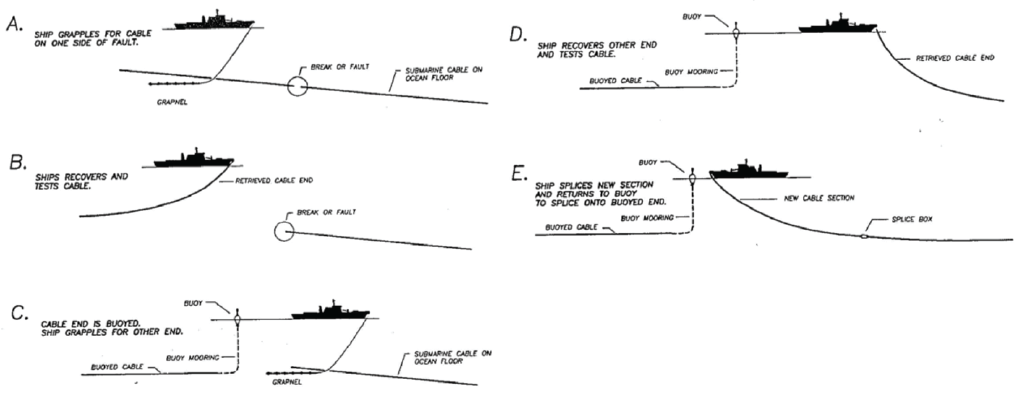
\includegraphics[width=14.17in]{figs/cable-repair-process} \caption{Ship operations for submarine cable repair. The ship runs a grapnel along the seafloor to catch the cable before the break, recovers and buoys one end of the cable, grapples and recovers the other, and splices a new section of repaired cable before laying it back onto the seafloor. Source: Tyco Electronics Subsea Communications, LLC}\label{fig:figSubmarineCableRepair}
\end{figure}

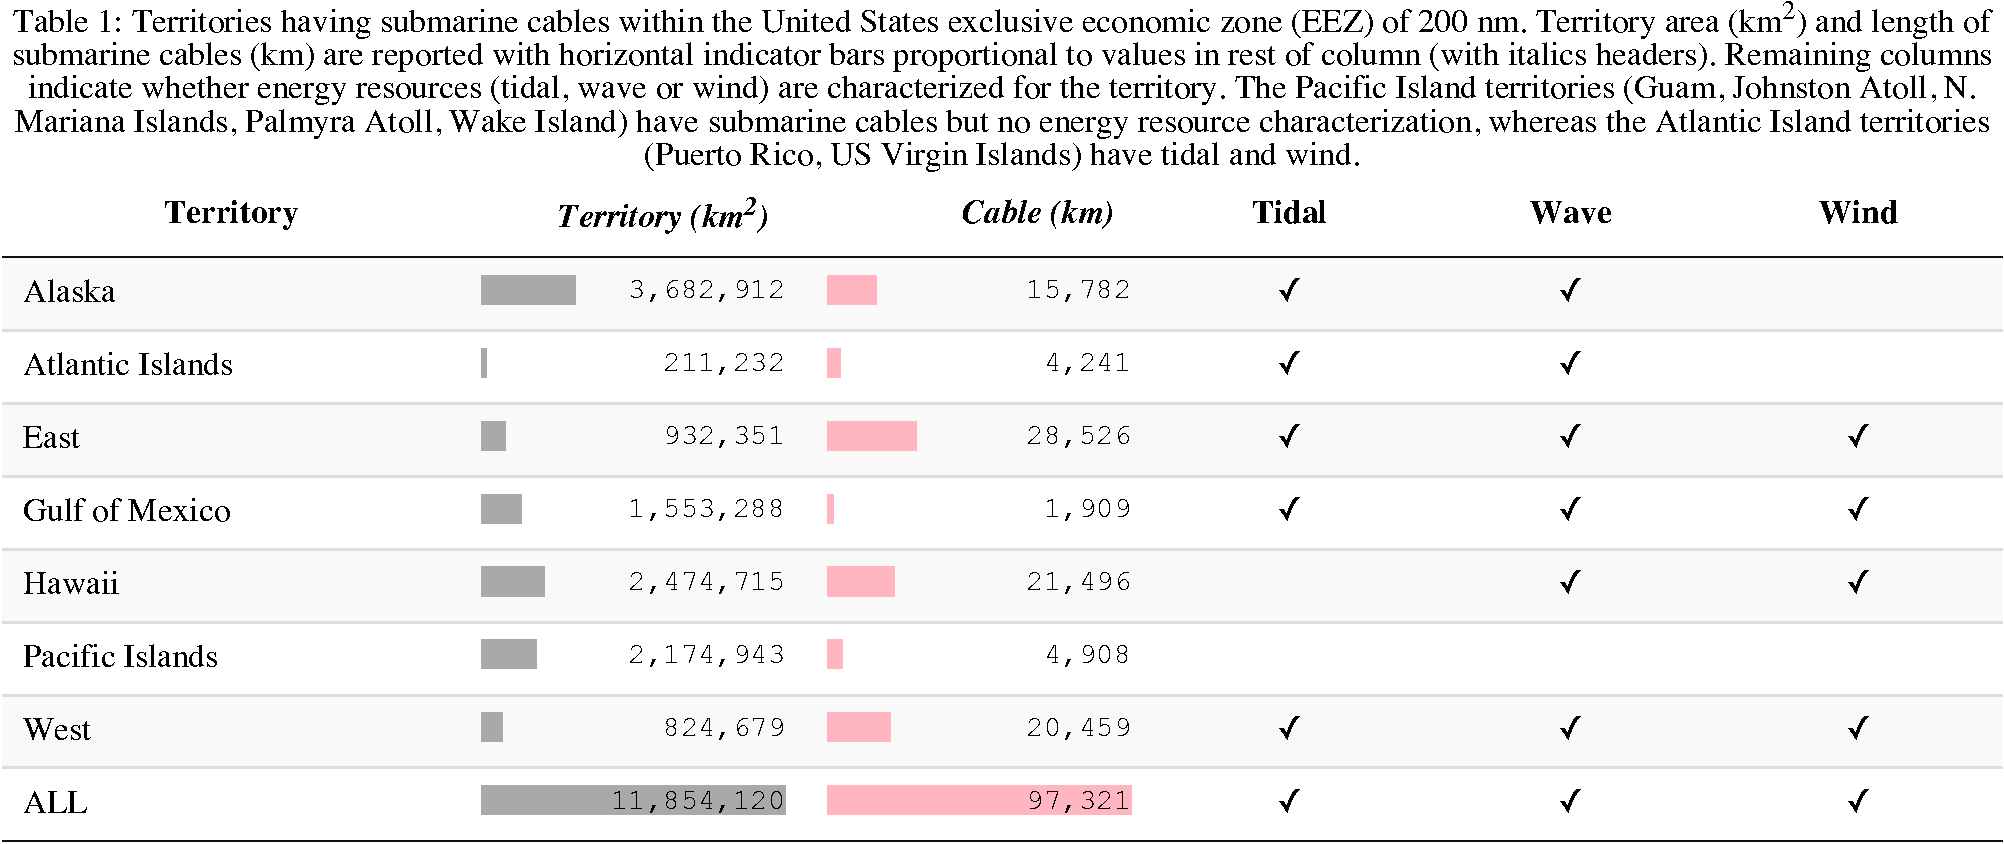
\includegraphics{report_tmp2_files/figure-latex/tbl01Territories-1.pdf}

\hypertarget{refs}{}
\hypertarget{ref-communicationssecurityreliabilityandinteroperabilitycounciliv_protection_2014}{}
Communications Security, Reliability and Interoperability Council IV.
(2014). \emph{Protection of Submarine Cables Through Spatial
Separation}.
\url{http://transition.fcc.gov/pshs/advisory/csric4/CSRIC_IV_WG8_Report1_3Dec2014.pdf}


\end{document}
